\chapter{Gradient Ascent}
\label{cha:gascent}
\section{Konzept}

Mit Zugriff auf die berechneten Gradienten des Modells, können diese verwendet werden um gezielt Bilder zu verändern. Dieses Verfahren wird als \textit{Gradient Ascent bezeichnet}, welches als Pendant zum Gradient Descent, einem Verfahren zum Training von neuronalen Netzen, verstanden werden kann. Demnach bedeutet der Ascent (dt. Aufstieg), dass die Eingabe verändert wird, um die Funktion und Neuronenaktivierung zu maximieren. Mithilfe einer \textit{targeted Backpropagation} werden demnach die Gradienten berechnet, die zum erreichen einer Zielausgabe (sprich Klasse) am relevantesten sind. Die Gradienten werden dann von dem ursprünglichen Bild (üblicherweise Zufallsgeneriert) mit einem Skalierungsfaktor mathematisch subtrahiert. Dabei kann man beobachten, dass relevante Pixel stärker mutiert werden und unwichtige Pixel weitgehend unverändert bleiben.

Die Methode sollte nach aussage von Ngunyen et al. \cite{nguyen_deep_2015} auf für selbst ausgewählte "'echte"' Bilder funktioniere. Um jedoch die Erkennbarkeit der ursprünglichen Bildes zu erhalten, sollten kleinere Skalierungsfaktoren verwendet werden. So wird ein "'über das Ziel hinausschießen"' verhindert und nur so gering wie nötig abgeändert, benötigt dann allerdings auch mehr Iterationsdurchläufe.
Diese Implementation wurde allerdings nicht weiter verfolgt, da das Konzept auch mit Zufallsbildern bestätigt werden konnte.

\section{Implementierung}
Der verwendete Code zur Erzeugung der Schadbilder mithilfe des Gradient Ascent Verfahrens basiert auf einer modifizierten Version von \cite{ozbulak_pytorch_2019}. Desweiteren wird ein angepasstes Modell basierend auf der AlexNet Architektur verwendet, mit Eingabedimensionen $64\times64\times3$ und einer Softmax Ausgabe von den 43 Klassen des \ac{GTSRB} Datensatz. 
Dieser Datensatz wurde für ein Training des \ac{NN} verwendet. 
Die final verwendete Version unseres AlexNet erreichte in der Validierung eine Genauigkeit von 0.89


Es wird ein zufälliges Bild erzeugt, welches als Eingabeparameter für das trainierte NN verwendet wird. 
Daraus werden durch Anwendung der \textit{categorical cross entropy} die Gradienten entsprechend für eine Zielklasse berechnet. Diese Gradienten werden nicht verwendet um die Parameter des NN zu ändern (wie es beim Training der Fall wäre), sondern um das eingegebene Bild gezielt zu modifizieren, indem die entsprechenden Pixel der aktivierten Neuronen je nach Aktivierungsstärke den Pixelwerten addiert werden.
Dieser Prozess wird iterativ wiederholt, bis das veränderte Bild die gewünschte Mindestkonfidenz einer ausgewählten Klasse erreicht hat. 

Die verwendete Implementation modifiziert Bilder, bis im lokalen \ac{NN} eine Konfidenz von 1 erreicht wurde. Diese Bilder werden im darauffolgenden Schritt an das Blackbox Modell gesendet und klassifiert. 

Ergebnisbilder mit einer Konfidenz >0.9 für irgendeine Klasse, wurden in eine gesonderte Textdatei mit Referenz auf den Speicherort, die erkannte Klasse und zugehörige Konfidenz abgespeichert.

%
%Generierung eines zufallsbildes (random noise)
%iterativer ablauf: 
%prediction
%gradienten berechnung durch kreuzentropie zur gewünschten klasse
%modifikation des bildes durch anteil der gradienten 
%

\section{Ergebnisse}
Als Ergebnis des Algorithmus wurden 43 Bilder respektive der 43 Klassen des letzten Layers erzeugt. Die Evaluation am zu überlistenden \ac{NN} ergab Konfidenzen >0.9 für 20 der 43 Bilder. Durch die Ähnlichkeit zwischen verschiedenen Klassen bzw. Straßenschildern, beispielsweise Höchstgeschwindigkeit 30 und 50, wurden nur 10 verschiedene Klassen in den 20 "'erfolgreichen"' Bildern erkannt.
Nachfolgende Grafiken \ref{tab:gasc1} zeigen verschieden Beispiele für die erzeugten Bilder mit initialen Zufallswerten. Wieder kam es zu Ergebnissen, welche eine andere Klasse lieferten, als für die Erzeugung verwendet wurde. Das für die Klasse \textit{Links Abbiegen} erzeugte Bild wurde vom Trasi-\ac{NN} beispielsweise als \textit{Kreisverkehr} erkannt.

\begin{table}
	\centering
\begin{tabular}{p{4.4cm}p{4.4cm}}
	\centering
	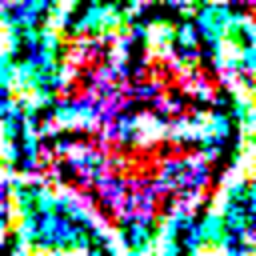
\includegraphics[width=\linewidth]{Images/AnPe/17_Einfahrtverbot} &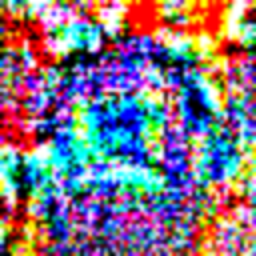
\includegraphics[width=\linewidth]{Images/AnPe/34_kreisverkehr_origTurnleft}  \\
	Einfahrt Verboten & Kreisverkehr \\
	0.9999&0.9535\\
	& (Ursprünglich als Links abbiegen erzeugt)\\
	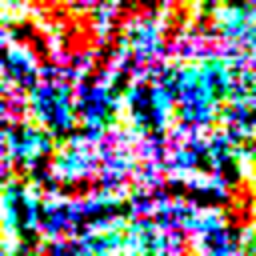
\includegraphics[width=\linewidth]{Images/AnPe/39_RechtsVorbeiOrigLinksvorbei} &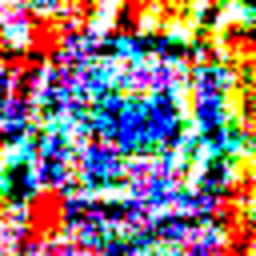
\includegraphics[width=\linewidth]{Images/AnPe/40_kreisverkehr}  \\
	Rechts Vorbei& Kreisverkehr\\
	0.9950&0.9868\\
\end{tabular}

\caption{Beispiele für Irrbilder mit Konfidenz >0.9}
\label{tab:gasc1}
\end{table}

Abschließend kann bestätigt werden, dass das Gradient Ascent verfahren die erzeugung von Täuschungsbildern ermöglicht. Einschränkungen des Verfahrens belaufen sich auf die Architektur und Ähnlichkeit des \ac{NN}. Es steht die Annahme, dass das verfahren mit größeren Bildern bessere Ergebnisse liefert.